\documentclass[runningheads]{llncs}
\usepackage{graphicx}
\usepackage{amsmath,amssymb} % define this before the line numbering.
\usepackage{ruler}
\usepackage{color}
\usepackage{subfig}
\usepackage[width=122mm,left=12mm,paperwidth=146mm,height=193mm,top=12mm,paperheight=217mm]{geometry}
\usepackage[pagebackref=true,breaklinks=true,colorlinks,bookmarks=false]{hyperref}
\begin{document}
% \renewcommand\thelinenumber{\color[rgb]{0.2,0.5,0.8}\normalfont\sffamily\scriptsize\arabic{linenumber}\color[rgb]{0,0,0}}
% \renewcommand\makeLineNumber {\hss\thelinenumber\ \hspace{6mm} \rlap{\hskip\textwidth\ \hspace{6.5mm}\thelinenumber}}
% \linenumbers
\pagestyle{headings}

% Definitions
\newcommand{\argmax}{\operatornamewithlimits{argmax}}
\def\subsectionautorefname{section}
\definecolor{light-gray}{gray}{0.3}
\newcommand{\aside}[1]{\textcolor{light-gray}{\emph{#1}}}
\newcommand{\todo}[1]{\textcolor{red}{\emph{#1}}}
\newcommand{\comment}[1]{}

\mainmatter
\def\ECCV12SubNumber{***}  % Insert your submission number here

\title{Timely Object Detection}

\titlerunning{ECCV-12 submission ID \ECCV12SubNumber}

\authorrunning{ECCV-12 submission ID \ECCV12SubNumber}

\author{Anonymous ECCV submission}
\institute{Paper ID \ECCV12SubNumber}

\maketitle

\begin{abstract}
\end{abstract}

\section{Sequential Decision Problem} \label{sec:sdp}

We first describe the requirements for our target system, and set the notation.
Details of our implementation are then given.

\subsection{Problem Setting} \label{sec:problem_setting}

We deal with a dataset of images $\mathcal{D}$, where each image $\mathcal{I}$ contains at least one, and often multiple, objects.
Each object is labeled with exactly one category label $1$ through $K$.

The multi-class, multi-label \emph{classification} problem asks whether $\mathcal{I}$ contains at least one object of class $i$, for each class $i \in \{1,\dots,K\}$.
The answer for a single label is given with a real-valued confidence by a function $\emph{classify}(\mathcal{I},i)$.
We write the ground truth for an image as $\mathbf{C}=\{C_1,\dots,C_K\}$, where $C_i \in \mathbb{B} = \{0,1\}$ is set to $1$ if an object of class $i$ is present.

The answer is evaluated by plotting precision vs. recall across dataset $\mathcal{D}$ (by progressively lowering the confidence threshold for a positive label) and integrating to yield the Average Precision (AP) metric \cite{pascal-voc-2010}.

We can make the classification problem more difficult by posing the \emph{counting} problem, which asks how many objects of class $i$ are present in $\mathcal{I}$, for each $i$.
This setting is not commonly evaluated; we mention it for its usefulness in later exposition.

Finally, the \emph{detection} problem is to output a list of bounding boxes (sub-images defined by four coordinates), each with a real-valued confidence that it encloses a single instance of an object of class $i$.
The answer for a single class $i$ is given by an algorithm $\emph{detect}(\mathcal{I},i)$, which outputs a list of bounding boxes $B$ and associated confidences.
To highlight the hierarchical structure of these problems, we note that the confidences may be given by $\operatorname{classify}(b,i)$ for each sub-image $b \in B$, and that the correct answer to the detection problem also answers the counting and classification problems.

Here we describe the classification problem setup, although we evaluate performance on both classification and detection tasks.

\subsection{Multi-class Classification Policy}

\begin{table}
\centering
\caption{Summary of the notation used.}
\label{tab:notation}
\begin{tabular}{|l|l|}
	\hline
	$C_i$         & presence of class $i$ \\ 
	$K$           & number of object classes \\ 
	$t$           & time into episode \\ 
	$T_s$, $T_d$  & start and deadline times \\ 
	$\mathcal{A}$ & set of actions \\ 
	$b_j$        	& belief state at step $j$ \\ 
	$\pi$         & policy, $\pi(b) \mapsto a \in \mathcal{A}$ \\ 
	\hline
\end{tabular}\end{table}

\begin{figure}[h!]
\center{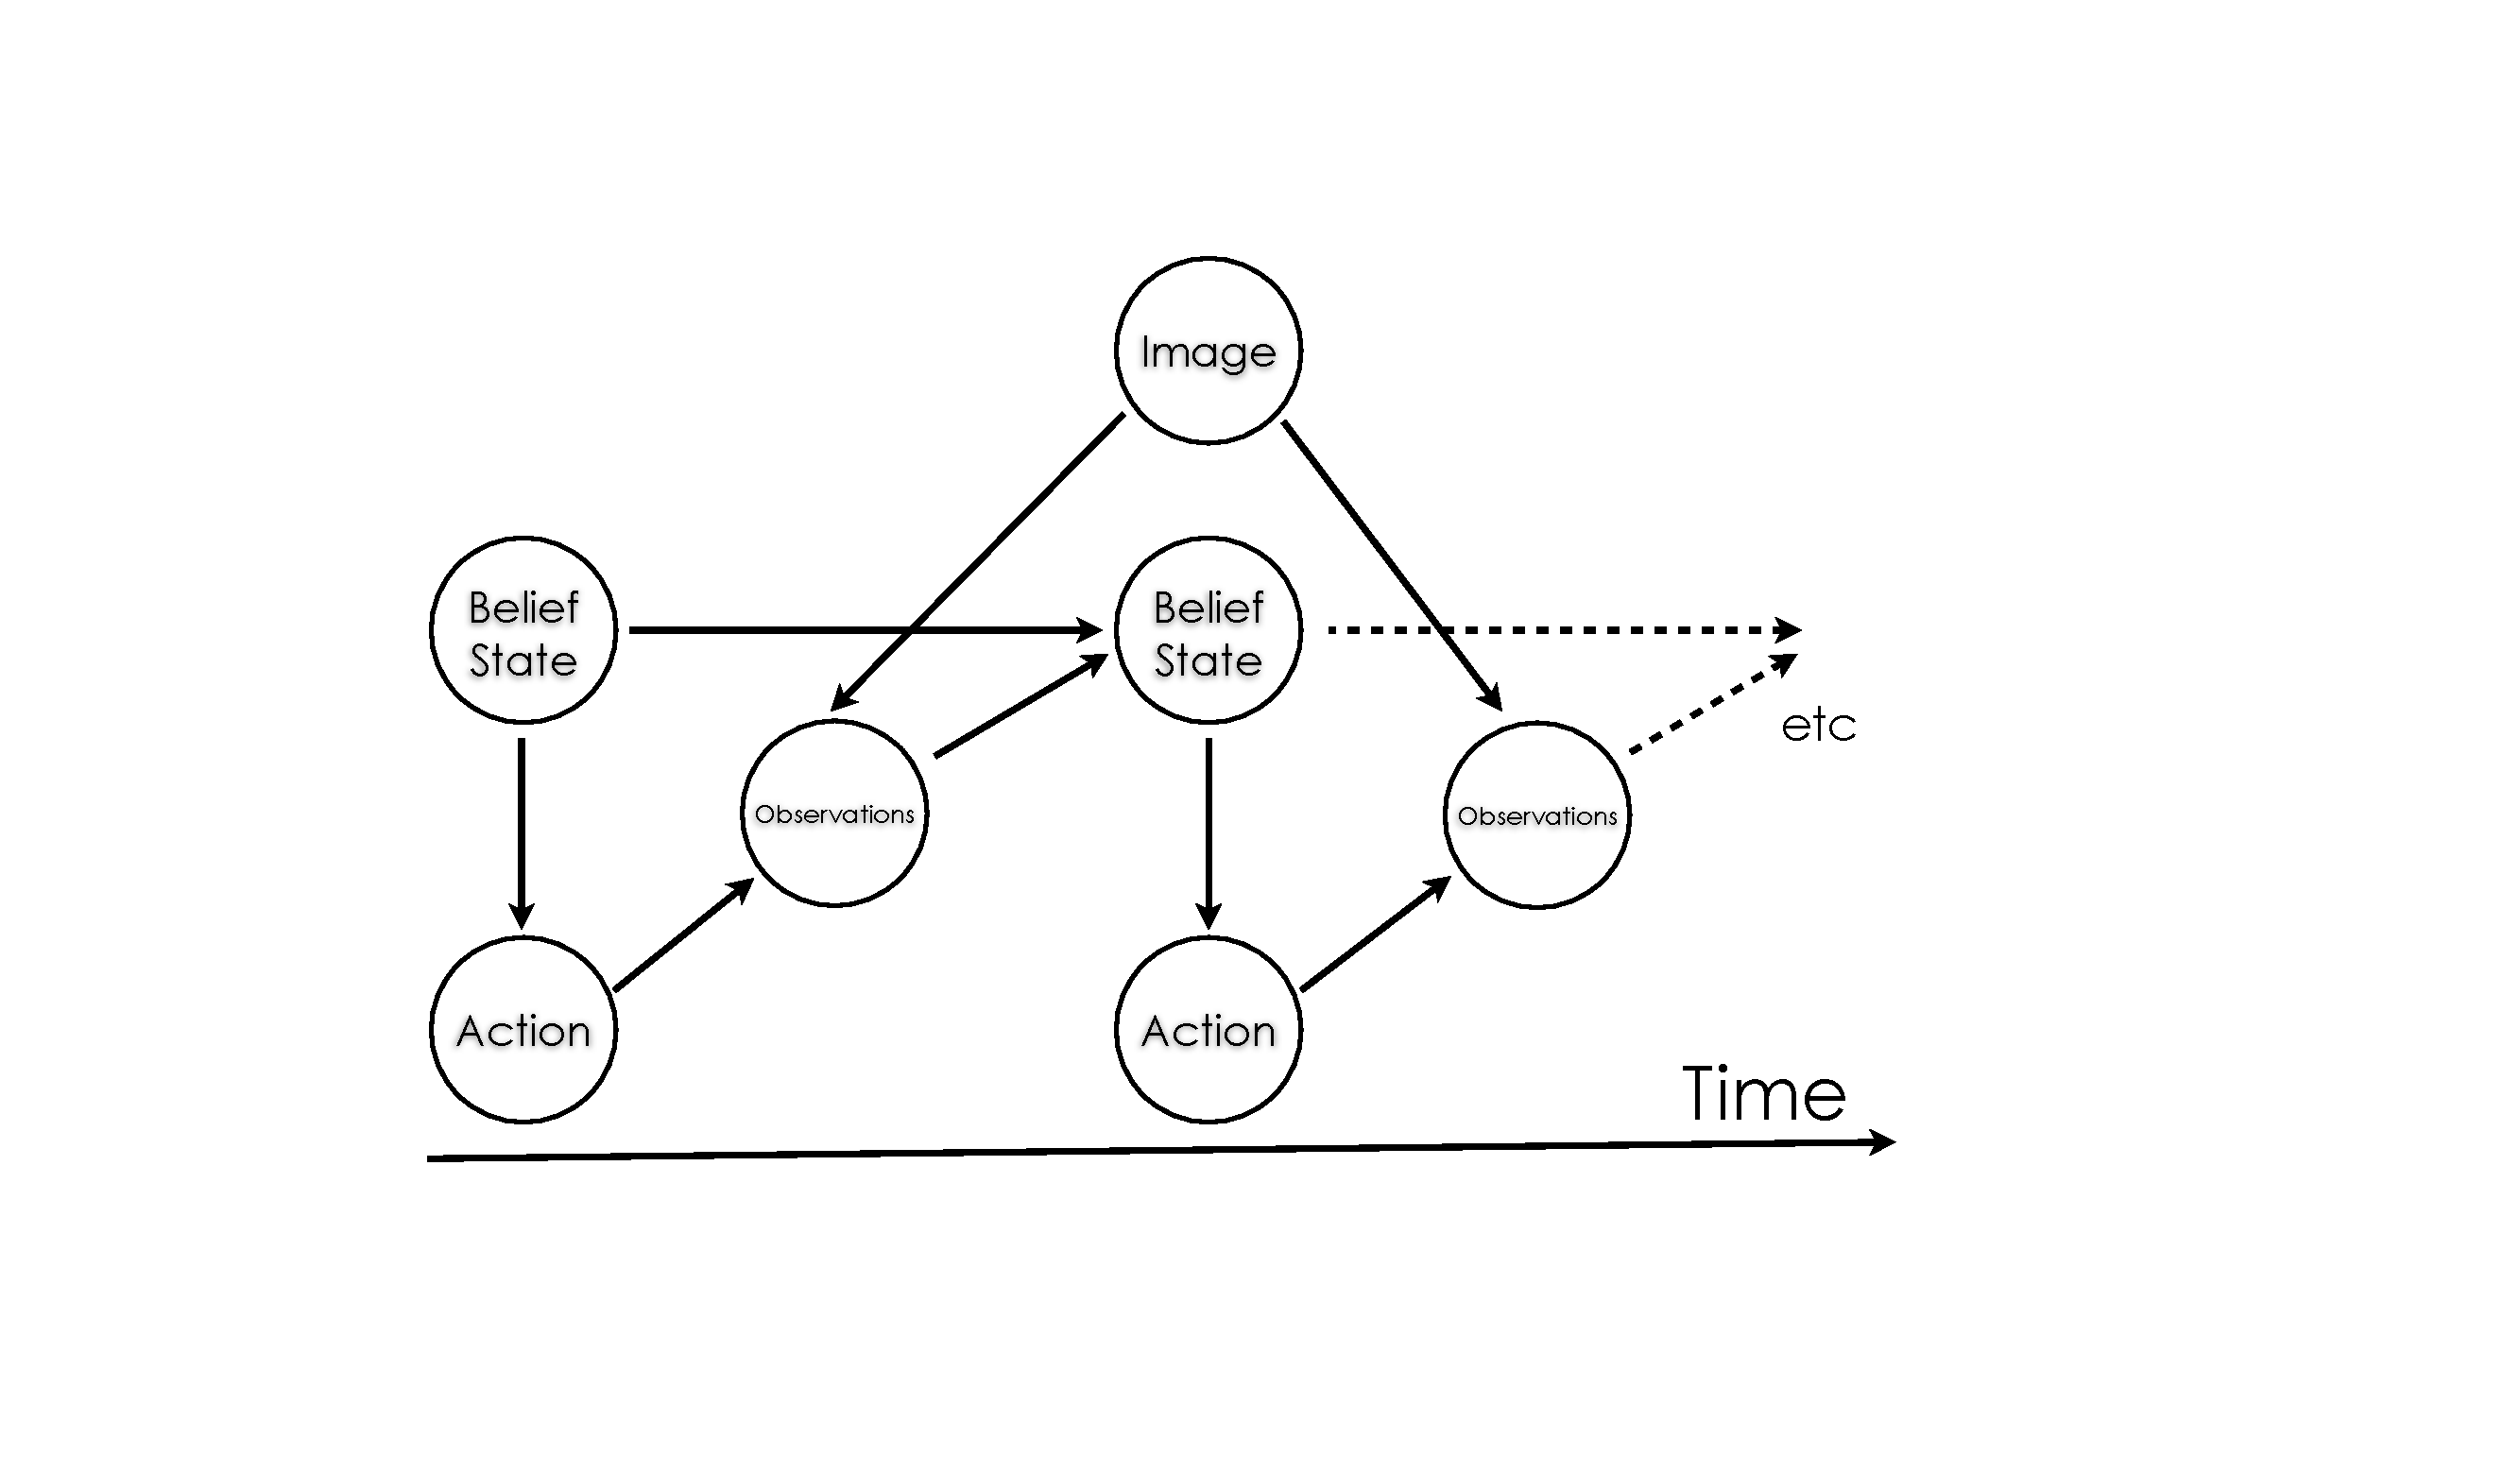
\includegraphics[width=0.66\linewidth]
    {figures/pomdp.pdf}}
  \caption{Summary of our approach to the problem. Our system has two major parts: (1) selecting an action by predicting its value; (2) updating the belief state with observations resulting from the action.}
  \label{fig:evaluation}
\end{figure}

Our goal is a multi-class classification policy $\pi$ that takes an image $\mathcal{I}$ and outputs $\{\emph{classify}(1), \dots, \emph{classify}(K)\}$.
The policy repeatedly selects an action $a$ from a set of actions $\mathcal{A}$, executes it, potentially receives a set of observations, and selects the next action.
A dynamic, or ``closed-loop,'' policy bases action selection on observations received from previous actions, exploiting the signal in inter-object and scene context for a maximally efficient path through the classifiers.
This is our goal, and what sets our formulation apart from multi-class systems that evaluate in a fixed order, such as simple cascades \cite{Viola2001} or \todo{add another one}.

The set of actions $\mathcal{A}$ can include per-class classifiers, ``scene context'' functions, and feature computations.
For simplicity of exposition, let $\mathcal{A}$ consist of $K+1$ feature computations $F$ and $2K$ per-class classifiers $L$:
\begin{itemize}
	\item $L^\text{co}_i$ are one-vs-all SVMs on a complex featurization of the image (computed by $F^\text{co}_i$);
	\item $L^\text{sc}_i$ are SVMs on a simple scene-level feature (computed by $F^\text{sc}$).
\end{itemize}

\todo{
Revise the above to make a single action compute all the scene classifiers at once.
}

Each classifier $L$ or feature computation $F$ has an expected cost $c(\cdot)$ of execution.
Depending on the setting, the cost can be defined in terms of algorithmic runtime analysis, an idealized property such as number of \emph{flops}, or simply the empirical runtime on specific hardware.
We take the empirical approach: every executed action advances $t$, the \emph{time into episode}, by its empirical runtime.

The system is given two times: the setup time $T_s$ and deadline $T_d$.
Between these times, the system must meet the goal of \emph{Anytime} performance and give the best possible answer to the classification problem at any point.

\begin{figure}[h!]
\center{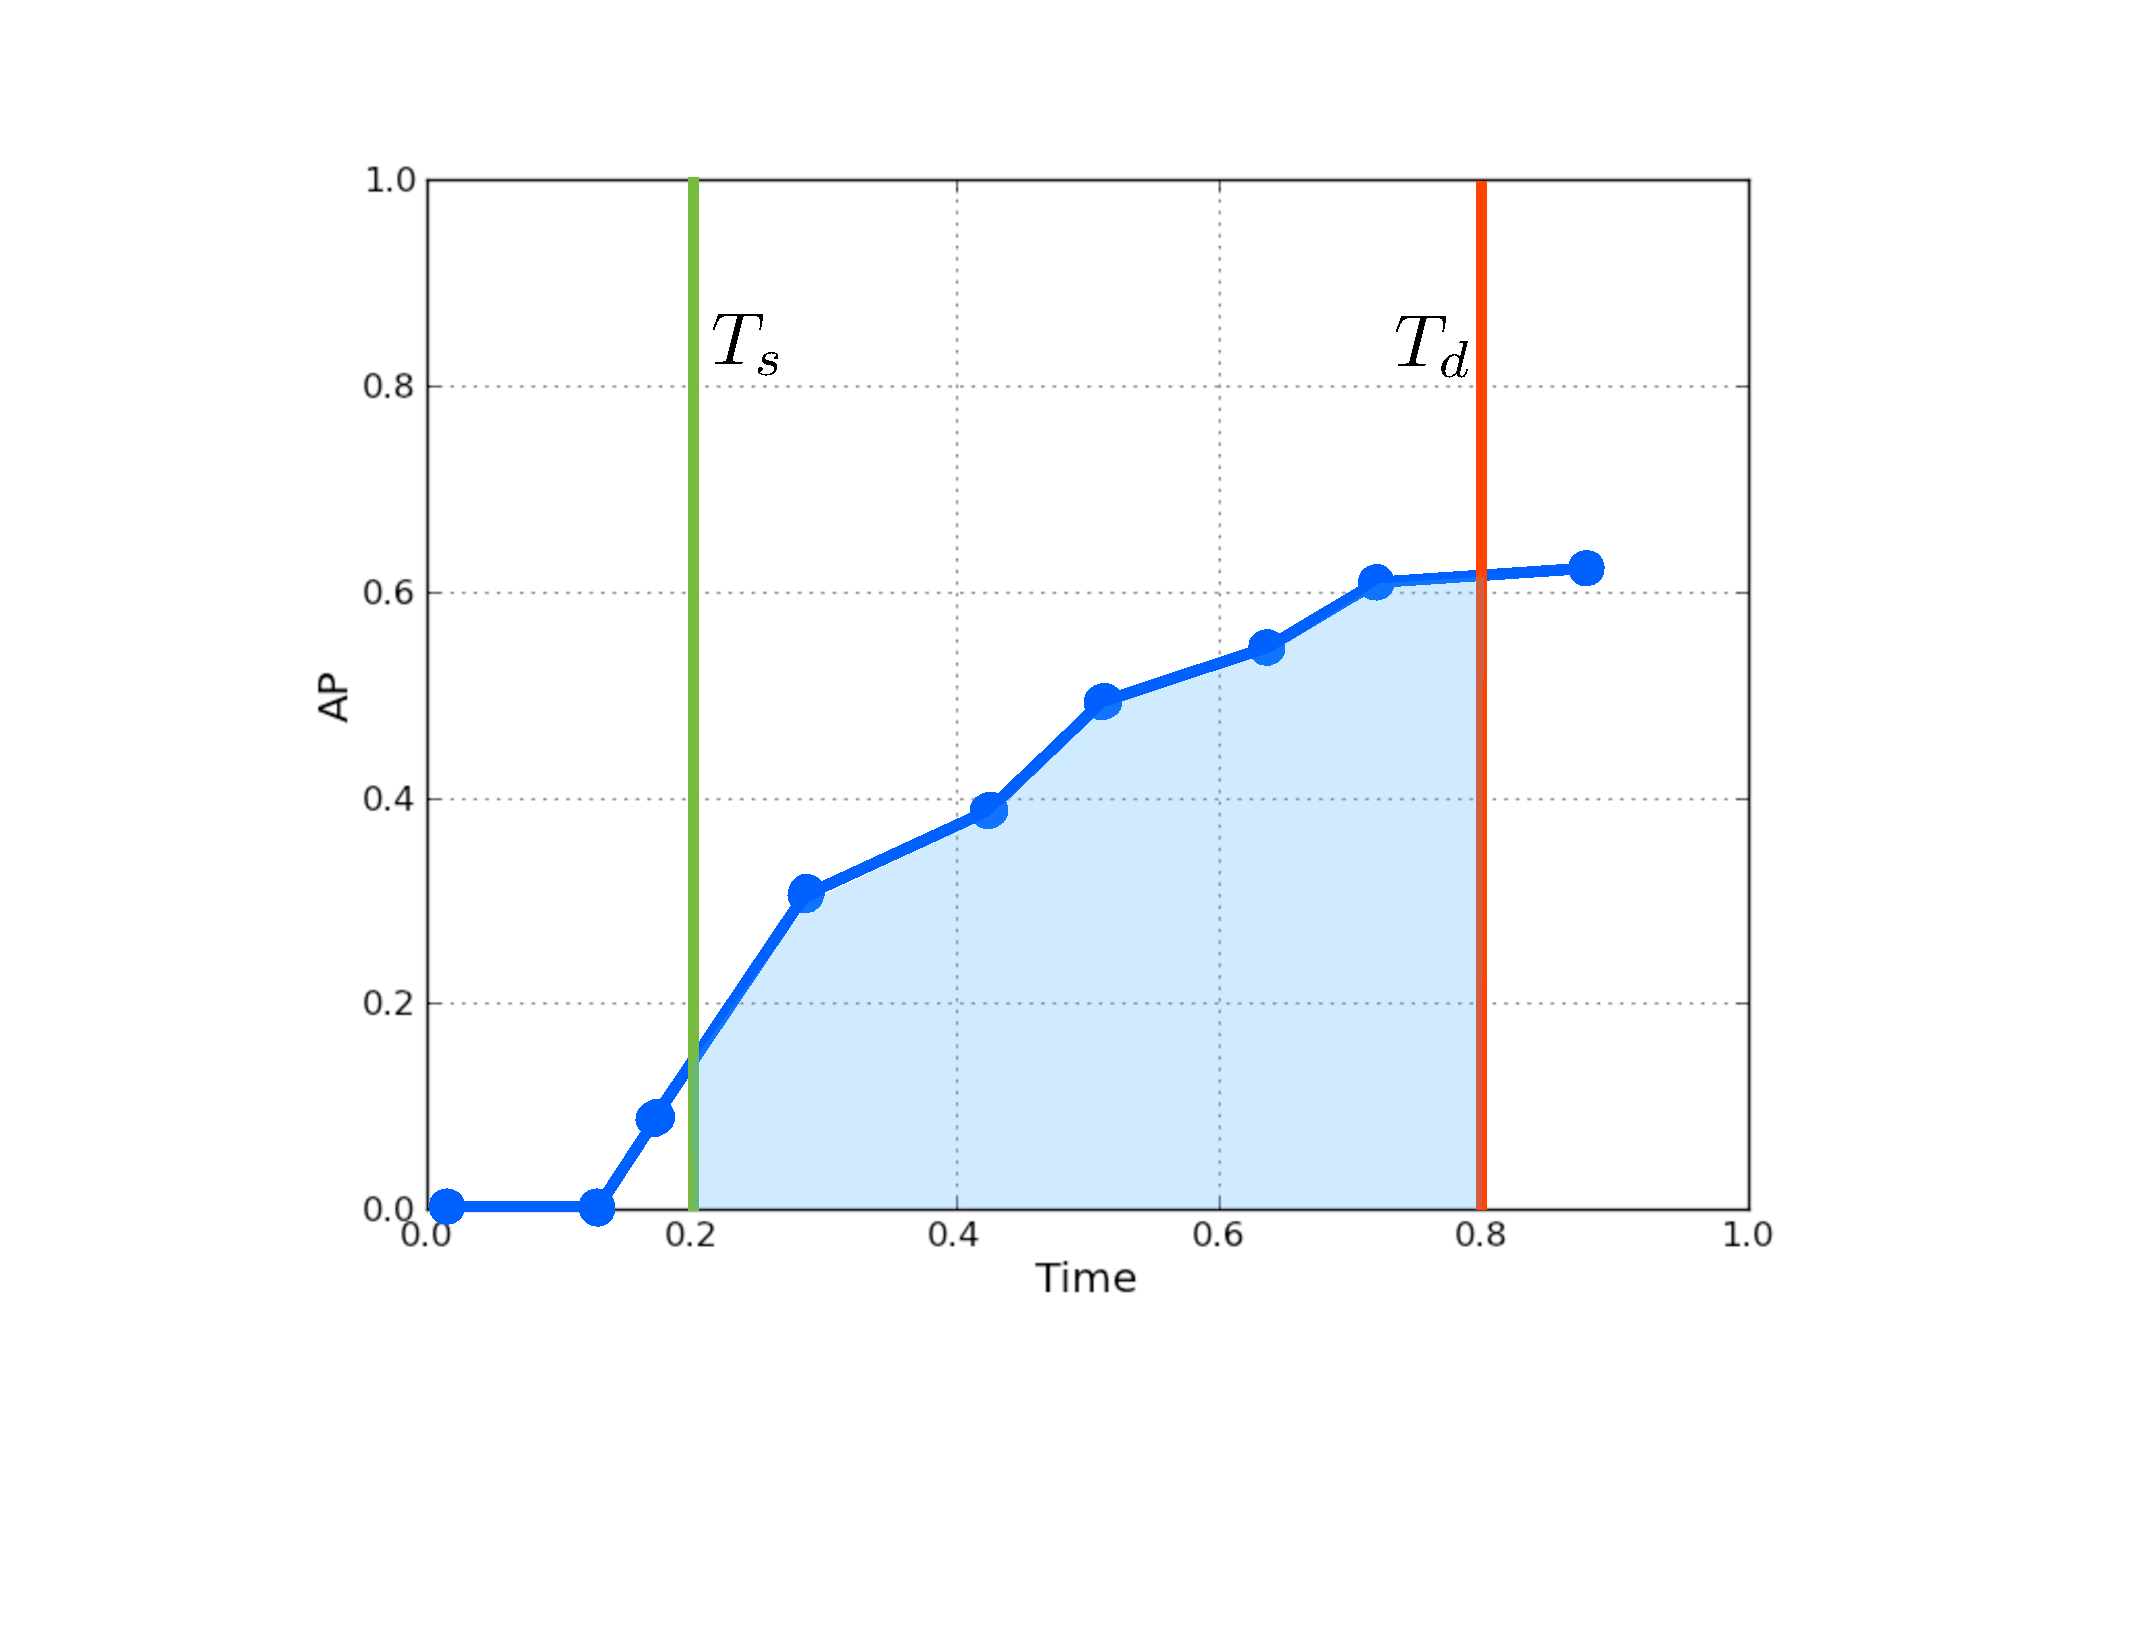
\includegraphics[width=0.66\linewidth]
    {figures/evaluation.pdf}}
  \caption{We aim for \emph{Anytime} performance within the bounds of the curve. That is, the policy should give the best possible answer at any time from start time $T_s$ to deadline $T_d$.}
  \label{fig:evaluation}
\end{figure}

To meet this goal, the evaluation metric of a policy is defined as the area under the performance vs. time curve between points $T_s$ and $T_d$ (see Figure~\ref{fig:evaluation}).
We evaluate policies by this more robust metric and not simply by the final performance at deadline time for the same reason---robustness---that Average Precision is used instead of a fixed Precision vs. Recall point.

We define the \emph{belief state} $b$ of the decision process by the the distribution over class presence variables $P(\mathbf{C}) = P(C_1, \dots, C_K)$ (writing $P(C_i)$ to mean $P(C_i=1)$), the time into episode $t$, the set of executed actions $\mathcal{O}$, and other variables that will be discussed in \autoref{sec:value}.
\comment{The terminology of ``belief'' comes from reinforcement learning and refers to the distribution $P(\mathbf{C})$.}

An action $a$ can result in a set of observations $o$ that are used to update the belief state.
At the very least, the state records the fact that $a$ has been taken by adding it to the initially empty set $\mathcal{O}$.

A classification \emph{episode} takes an image $\mathcal{I}$ and proceeds from the initial belief state $b_0$ and action $a_0$ to the next pair $(b_1,a_1)$, and so on until $t$ exceeds $T_d$.
At that point, the policy is terminated and a new episode begins on a new image.

The policy's performance is determined by treating the final values of $P(\mathbf{C})$ as the set of confidence scores $\{\emph{classify}(1), \dots, \emph{classify}(K)\}$ for the multi-label classification evaluation (see \autoref{sec:problem_setting}).

\subsection{The value function} \label{sec:value}
Optimal performance results from becoming maximally certain of the correct values $C_i$ as quickly as possible (given the setup time).
As our goal is to pick actions, we want to formulate a function that assigns a value to a potential action, given the current state of the decision process.
We will then be able to define our policy as simply
\begin{equation}
\pi(b) = \argmax_{a \in \mathcal{A} \setminus \mathcal{O}} V(b,a)
\end{equation}

We consider two formulations of the value function: one based on information gain, and one on the classification loss.

\subsubsection{Information gain}
negative residual entropy, following \cite{Gao2011}.

\todo{Write this out, and mention the greedy submodularity argument, to be made in a later section.}

\subsubsection{Classification loss}
\todo {Write this out. What to do with the cost here?}

\subsection{Updating the belief state}
While the value function can learn certain dependencies between class occurrences, its job is made easier if the belief state already presents features that clearly present the relevant signals, such as co-occurence.
Toward this end, we employ an inference model to infer the marginals $P(C_i)$ given the observations.
It may also be useful to predict the marginals $P(L_i)$, as some formulations of our value function make use of this information.

We explore two alternatives for the inference model: a fully-connected Markov Random Field (MRF) and a locally weighted regression, as shown in Figure~\ref{fig:models}.

\begin{figure}[h!]
\centering
\subfloat[MRF]{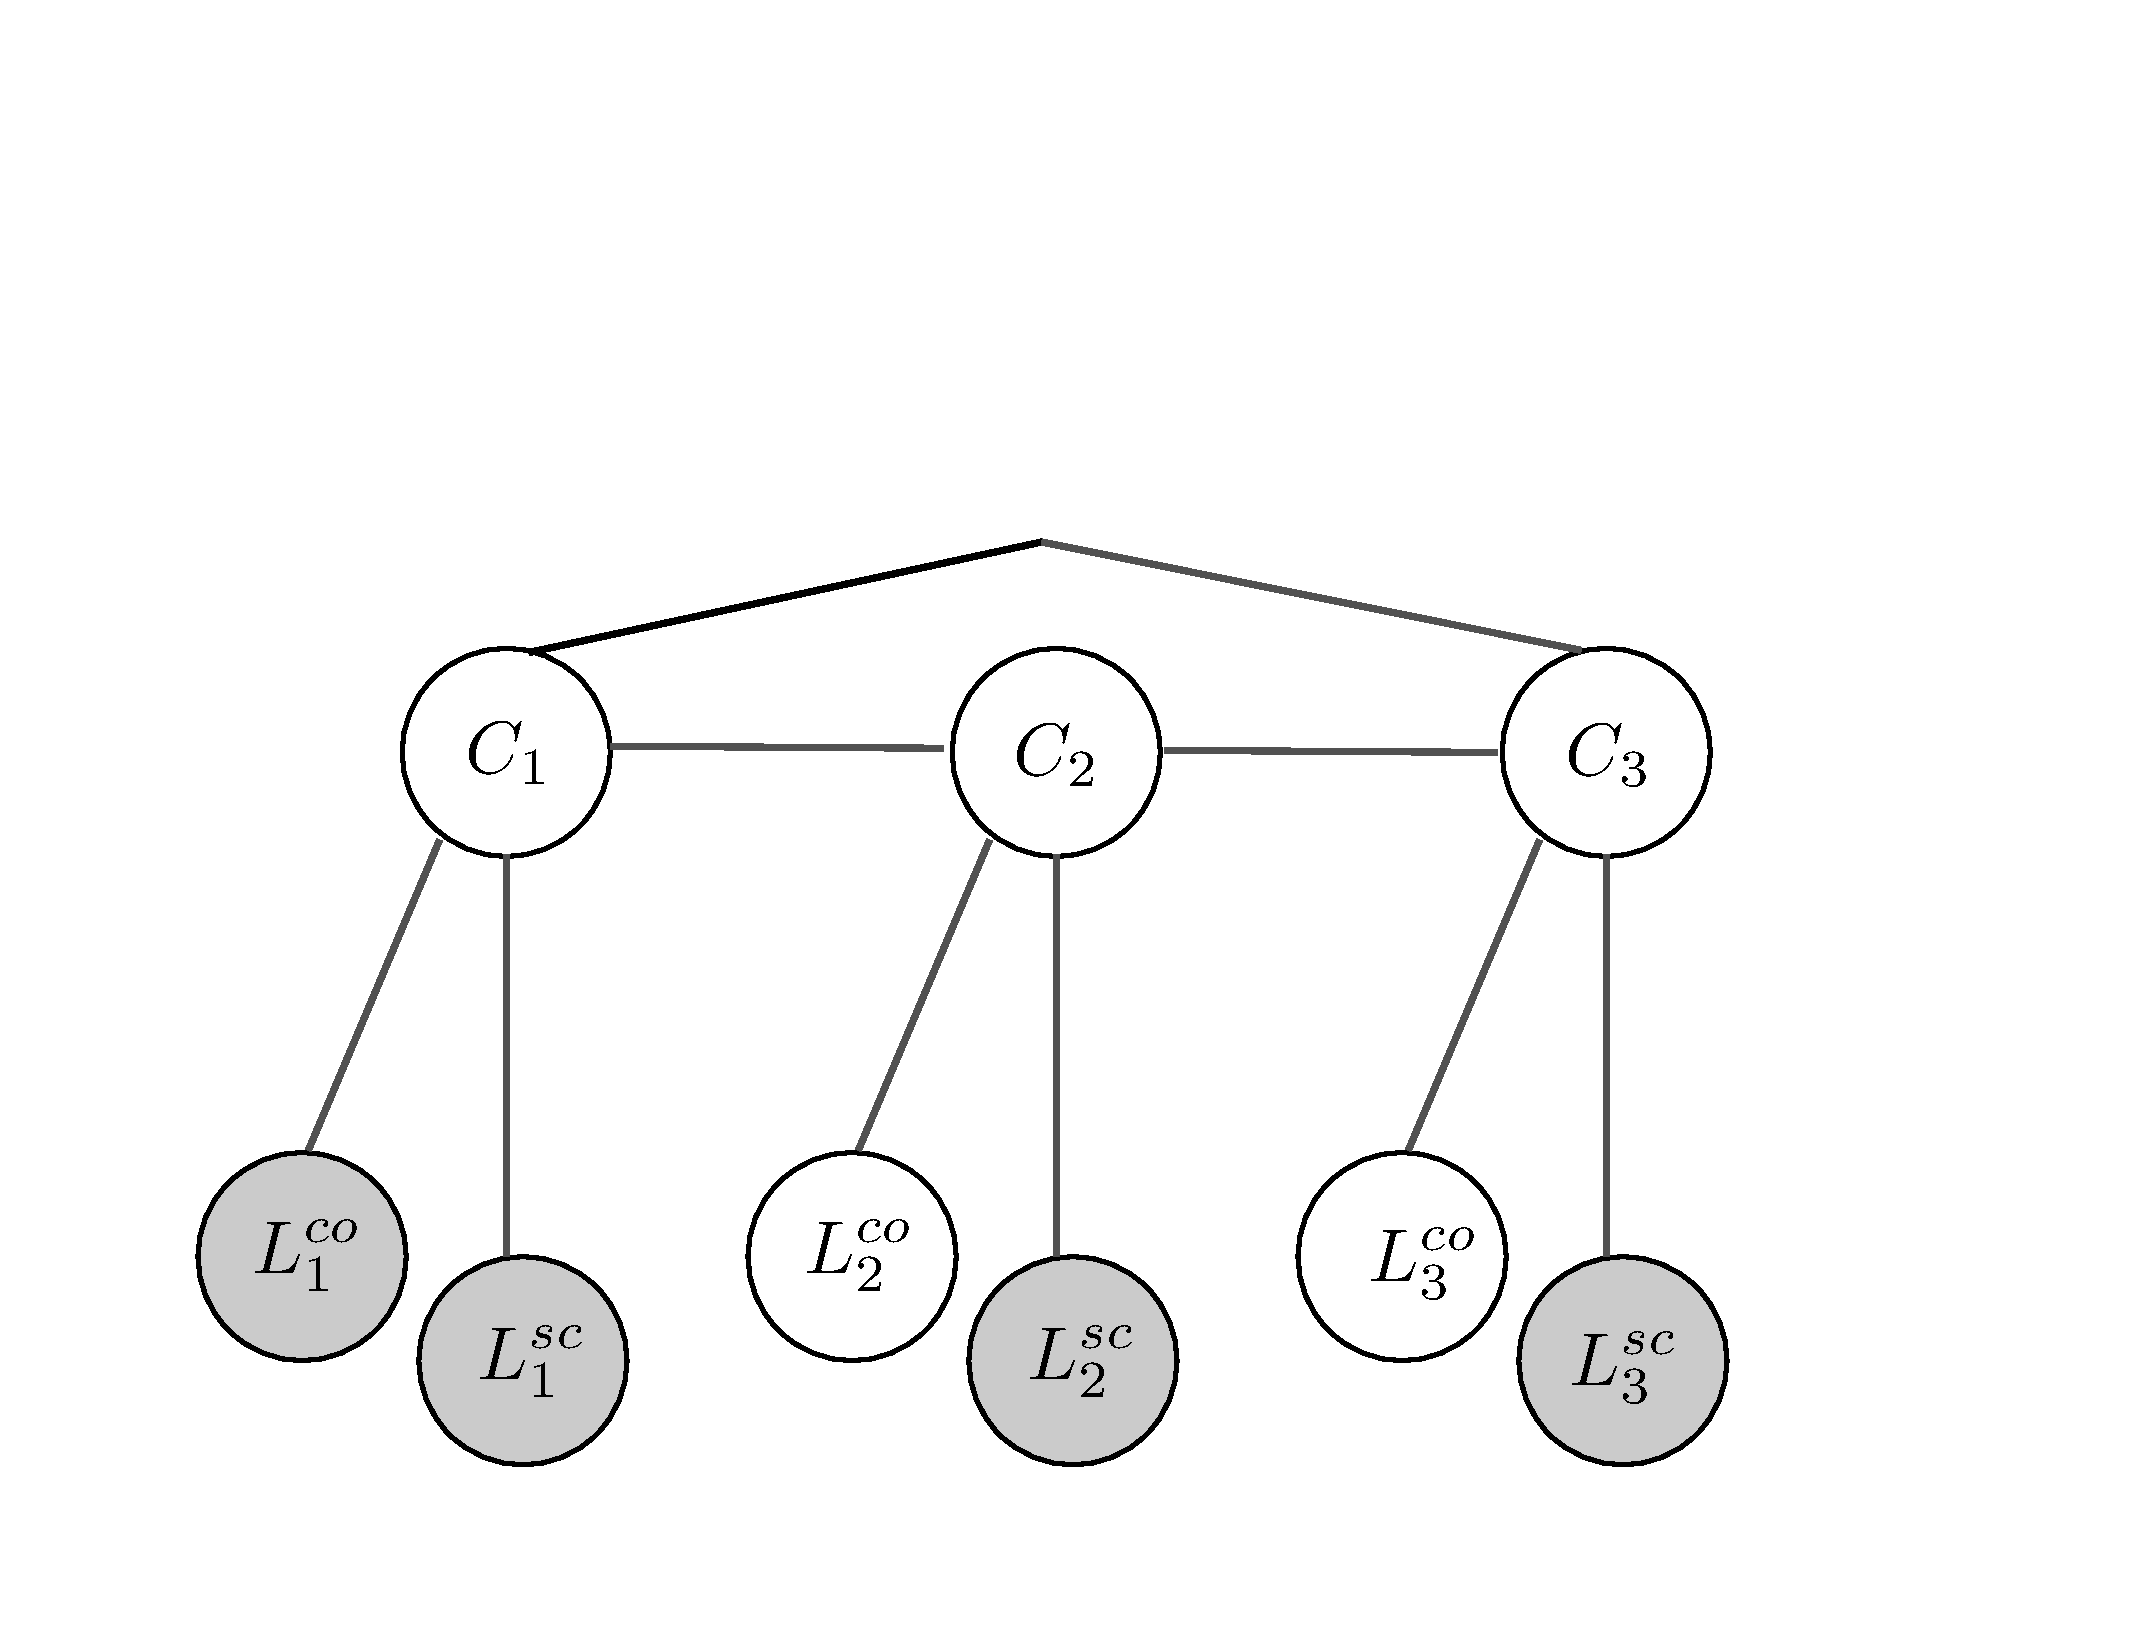
\includegraphics[width=0.46\linewidth]{figures/inf_model_mrf.pdf}} \hfill
\subfloat[Local]{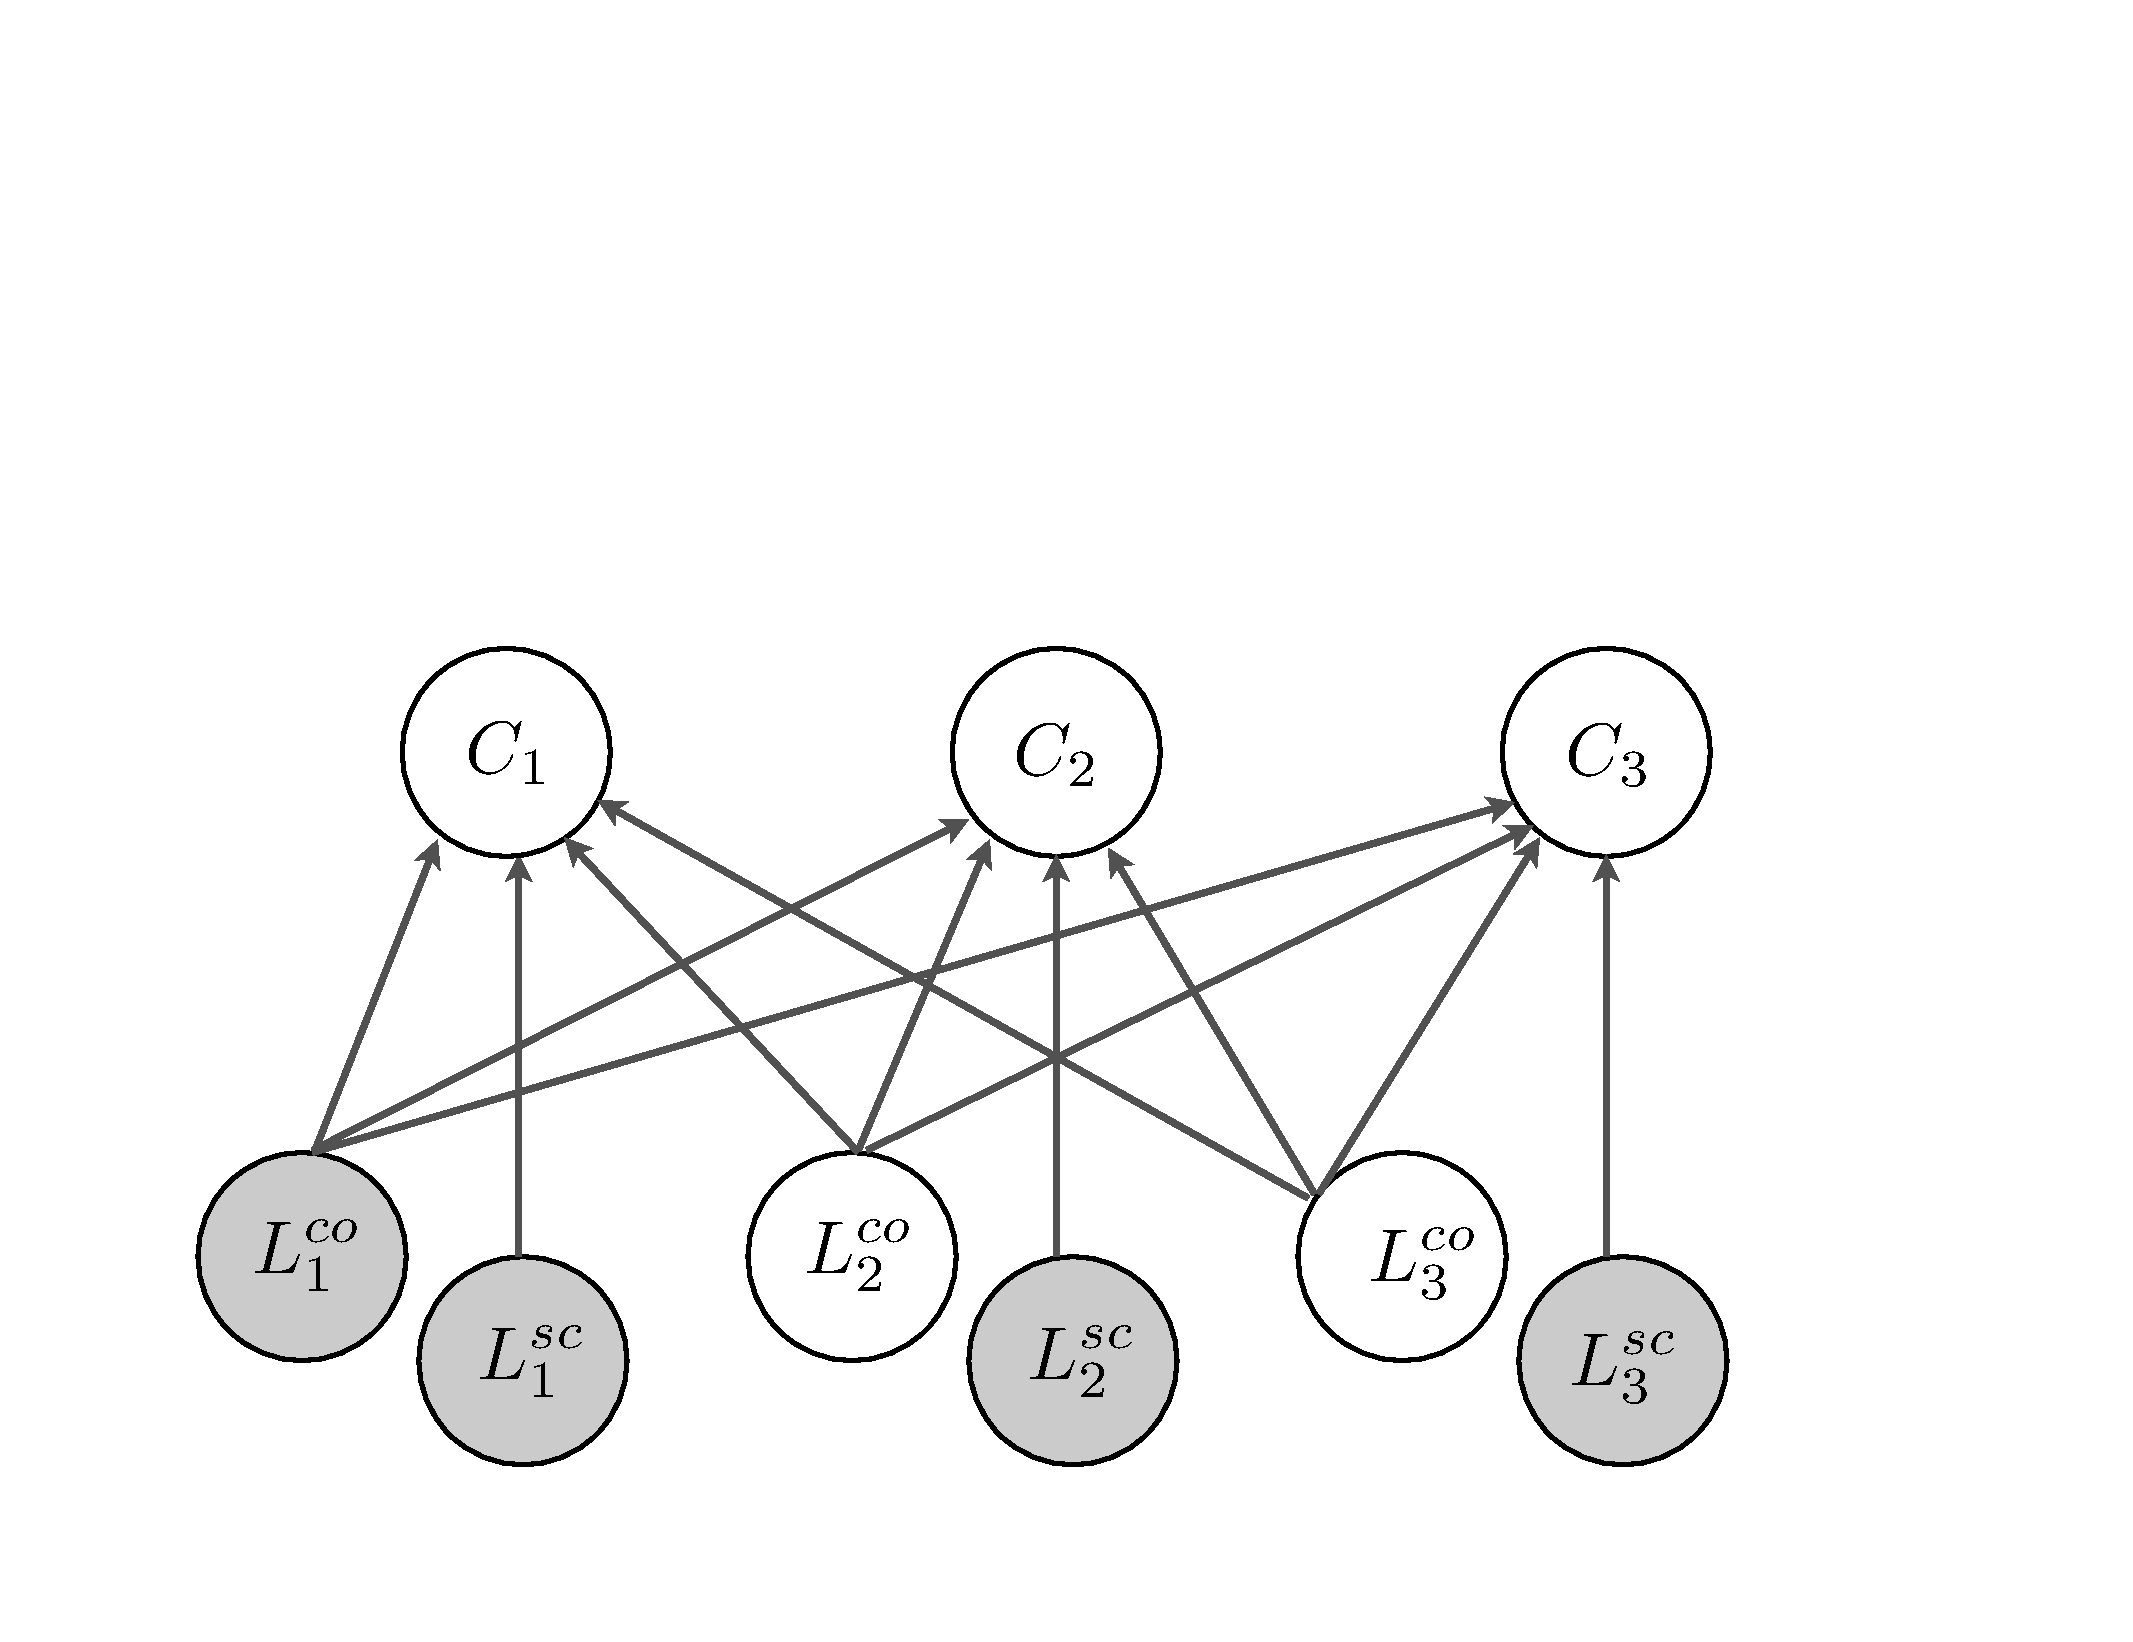
\includegraphics[width=0.46\linewidth]{figures/inf_model_loc.pdf}}
\caption{The models present a point in the middle of the decision process, when some classifiers have already been observed.}
\label{fig:models}
\end{figure}

\subsubsection{MRF inference}
Pros: (probably) more efficient at test time.

Cons: model too restrictive? not exact inference.

\subsubsection{Locally weighted regression}
Approach of \cite{Gao2011}.

Pros: imposing minimal model constraints (except Gaussian assumptions); 

Cons: expensive at test time; data too sparse?

\subsection{Reward} \label{sec:reward}
Let's say that given deadline $T_d$ and some image, the policy had time to take $J$ actions.
The total expected reward of a policy $\pi$ is then defined as the sum of rewards
\begin{equation}
\mathbb{E}_\pi[\sum_{j=0}^J R(b_j)]
\end{equation}

The reward function does not necessarily have to be related to the evaluation of the system.
We explore two options for the reward function: the first is derived directly from the evaluation metric; the second seeks to minimize entropy of $P(\mathbf{C})$.

\subsubsection{Slope of performance vs. time}
\begin{figure}[htb]
  \center{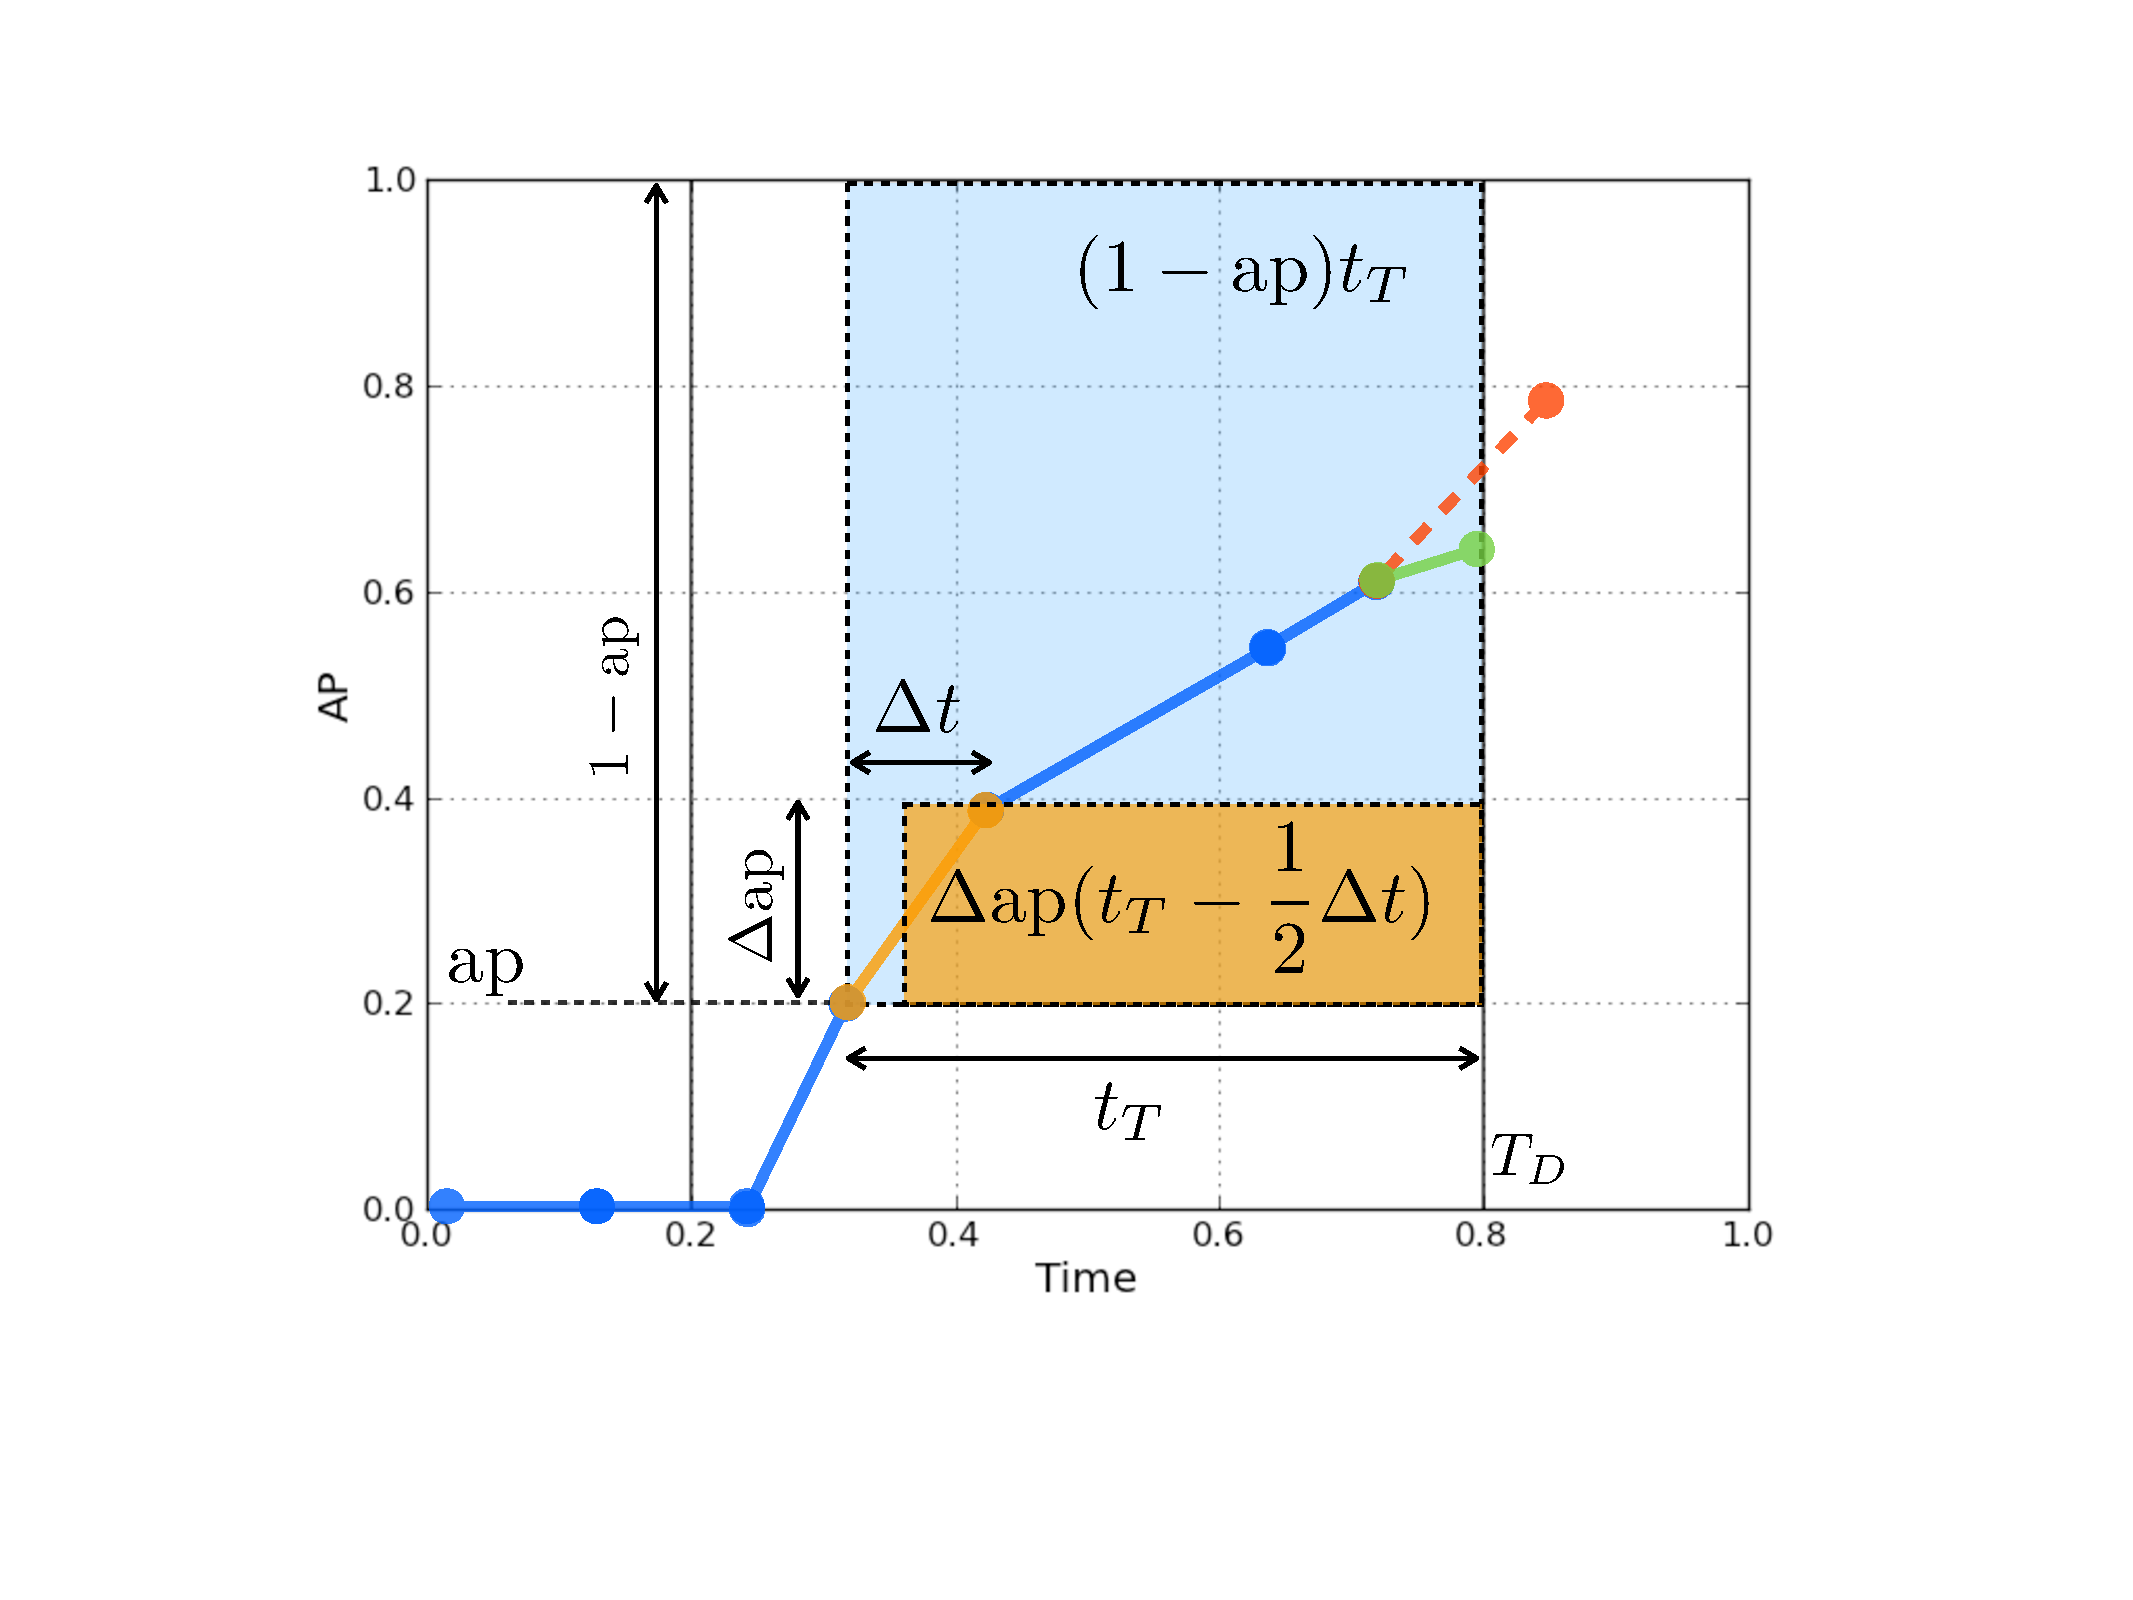
\includegraphics[width=0.66\linewidth]{figures/apvst_expl.pdf}}
  \caption{\label{fig:rewards}A per-action greedy value function that corresponds to the maximization of our objective function is the area of the horizontal slice under the curve due to the action. The figure shows this analysis for the action highlighted in orange.}
\end{figure}

Remembering that the final evaluation of a policy consists of the area under the performance vs. time curve, we formulate per-action rewards such that their addition results in precisely this quantity.
Specifically, as shown in Figure~\ref{fig:rewards}, we define the reward of an action as
\begin{equation}\label{eq:advanced}
\Delta AP (t_T-\Delta t)
\end{equation}
where $t_T$ is the time left until deadline, and $\Delta t$ and $\Delta AP$ are the time taken and AP change produced by the action.

The equation breaks down into a term to maximize, $\Delta AP t_T$, and a term to minimize, $\Delta AP \Delta t$.
This agrees with the intuition that to capture the most area under the curve, the slope needs to be maximized at each point.
Additionally, the equation shows that if $\Delta t$ exceeds $t_T$, the value of taking the action is negative.

At each step, we want to pick the action that maximizes the expected rewards until the end of the episode.
We therefore define our policy as
\begin{equation}
\pi(b) = \argmax_{a \in \mathcal{A} \setminus \mathcal{O}} \theta^\top \phi(b,a)
\end{equation}

Learning this accurately is the domain of Reinforcement Learning research, and is generally intractable for large-scale POMDPs.
We explore three different value functions.

First, we seek to maximize the expected next-stage reward, and manually construct a value function such that picking the action with maximal value achieves this.
Next, we note that the manually constructed value function can be represented as a scalar product of a parameter vector with a featurization of the belief state; we learn the weights by regression to the actual next-stage reward from running many episodes.
Lastly, we use a reinforcement learning technique to learn the weights such that the expected rewards over the whole episode are maximized.

\subsubsection{Greedy expected-value}
We can compute the expected value of the reward function given a distribution over the classifier response.
If we define the value function by this expectation, we will have constructed a one-step greedy policy.

\note{Discuss submodularity defense of greedy policies here; costs are tricky though.}

\subsubsection{Learning the greedy policy}
We note that we can represent the one-step greedy policy value function as a scalar product 

\subsubsection{Learning the proper policy}
\note{I'm considering two options here: (1) log-linear representation and policy gradient algorithm; (2) least-squares policy iteration.}

\paragraph{Policy gradient algorithm}
We redefine our policy as picking the mode of a log-linear parametrized distribution:
\begin{equation}
P(a|b;\theta) = \frac{\exp(\theta^T \phi(b,a))}{\sum_{a' \in \mathcal{A}} \exp(\theta^T \phi(b,a')}
\end{equation}

Basically stochastic gradient ascent on the estimate of the reward accrued by an episode.

This approach has been shown to scale to large problems in \cite{Branavan2009}, although it has been proven to converge only to local maxima and only for MDPs \cite{Sutton2000}.

\note{Does the constraint that no action is taken more than once affect this algorithm?}

\paragraph{Least-squares Policy Iteration}
An efficient form of temporal-difference learning used in \cite{Kwok2004}.
Policy remains parameterized as it was.

\section{Evaluation} \label{sec:evaluation}
- show that the greedy policy works better than random and better than fixed-order
- show that the reinfrocement learning policy works better than greedy, at least for the non-infogain rewards.

\subsection{Classification}

\subsection{Detection}
We also evaluate using the task of detection (see \autoref{sec:problem}).


\bibliographystyle{splncs}
\bibliography{sergeyk-bibtex}

\end{document}
